\section{Simulations}

% ERROR: Maybe this should be named something like "Applications to models"?

\subsection{Linear regression with known variance}

When variance is known, the left side reduces to a constant. This does not affect where the maximum of the information gain function is reached. This means that the left side can be dropped.

The equation

\begin{equation}
	ig(x) = h \left(\int p(y) \right)  - \int h \Bigl( p(y) \Bigl)
\end{equation}

becomes

\begin{equation}
	ig(x) = h \left(\int p(y) \right)
\end{equation}

The distribution of p(y) is a mixture of normal distributions, and consequently its entropy can not be solved in closed dorm.

\begin{figure}
	\begin{center}
		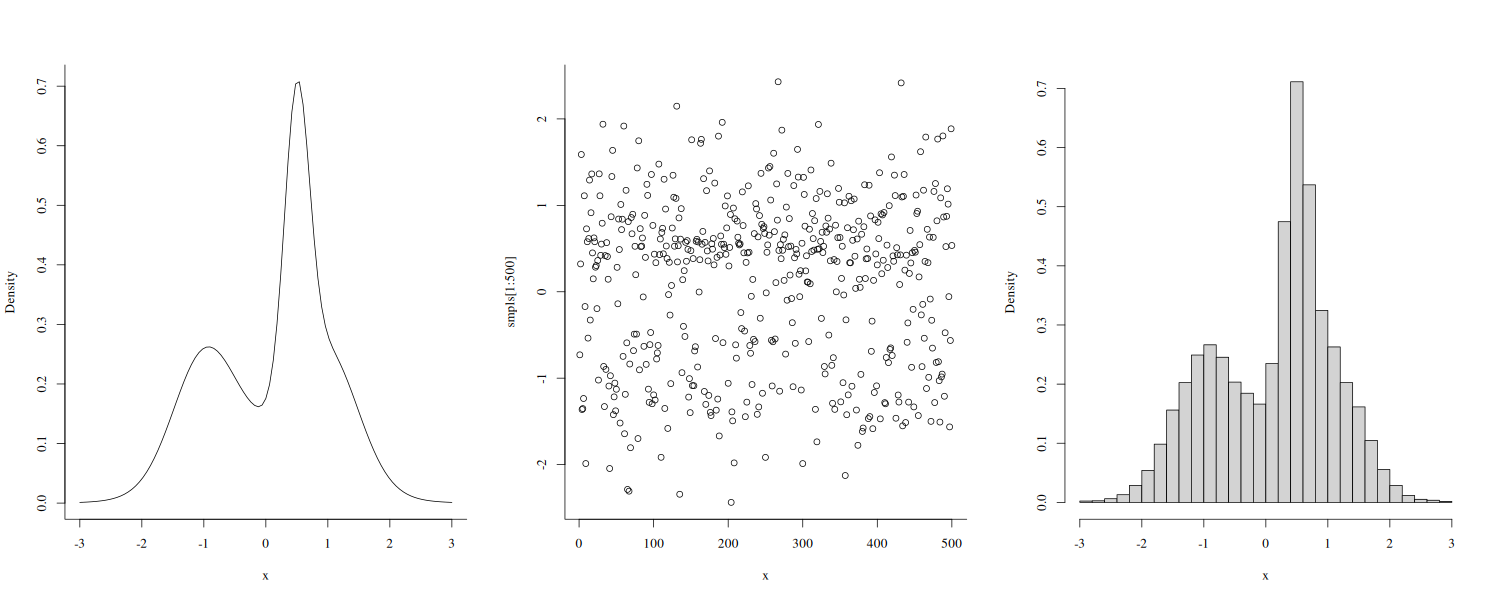
\includegraphics[width=5in]{Parts/TheoreticalBackground/Figs/etnropyApproxHist.png}
	\end{center}
	\caption{}
\end{figure}